% Options for packages loaded elsewhere
\PassOptionsToPackage{unicode}{hyperref}
\PassOptionsToPackage{hyphens}{url}
\PassOptionsToPackage{dvipsnames,svgnames,x11names}{xcolor}
%
\documentclass[
  super,
  preprint,
  3p]{elsarticle}

\usepackage{amsmath,amssymb}
\usepackage{iftex}
\ifPDFTeX
  \usepackage[T1]{fontenc}
  \usepackage[utf8]{inputenc}
  \usepackage{textcomp} % provide euro and other symbols
\else % if luatex or xetex
  \usepackage{unicode-math}
  \defaultfontfeatures{Scale=MatchLowercase}
  \defaultfontfeatures[\rmfamily]{Ligatures=TeX,Scale=1}
\fi
\usepackage{lmodern}
\ifPDFTeX\else  
    % xetex/luatex font selection
\fi
% Use upquote if available, for straight quotes in verbatim environments
\IfFileExists{upquote.sty}{\usepackage{upquote}}{}
\IfFileExists{microtype.sty}{% use microtype if available
  \usepackage[]{microtype}
  \UseMicrotypeSet[protrusion]{basicmath} % disable protrusion for tt fonts
}{}
\makeatletter
\@ifundefined{KOMAClassName}{% if non-KOMA class
  \IfFileExists{parskip.sty}{%
    \usepackage{parskip}
  }{% else
    \setlength{\parindent}{0pt}
    \setlength{\parskip}{6pt plus 2pt minus 1pt}}
}{% if KOMA class
  \KOMAoptions{parskip=half}}
\makeatother
\usepackage{xcolor}
\setlength{\emergencystretch}{3em} % prevent overfull lines
\setcounter{secnumdepth}{5}
% Make \paragraph and \subparagraph free-standing
\ifx\paragraph\undefined\else
  \let\oldparagraph\paragraph
  \renewcommand{\paragraph}[1]{\oldparagraph{#1}\mbox{}}
\fi
\ifx\subparagraph\undefined\else
  \let\oldsubparagraph\subparagraph
  \renewcommand{\subparagraph}[1]{\oldsubparagraph{#1}\mbox{}}
\fi

\usepackage{color}
\usepackage{fancyvrb}
\newcommand{\VerbBar}{|}
\newcommand{\VERB}{\Verb[commandchars=\\\{\}]}
\DefineVerbatimEnvironment{Highlighting}{Verbatim}{commandchars=\\\{\}}
% Add ',fontsize=\small' for more characters per line
\usepackage{framed}
\definecolor{shadecolor}{RGB}{241,243,245}
\newenvironment{Shaded}{\begin{snugshade}}{\end{snugshade}}
\newcommand{\AlertTok}[1]{\textcolor[rgb]{0.68,0.00,0.00}{#1}}
\newcommand{\AnnotationTok}[1]{\textcolor[rgb]{0.37,0.37,0.37}{#1}}
\newcommand{\AttributeTok}[1]{\textcolor[rgb]{0.40,0.45,0.13}{#1}}
\newcommand{\BaseNTok}[1]{\textcolor[rgb]{0.68,0.00,0.00}{#1}}
\newcommand{\BuiltInTok}[1]{\textcolor[rgb]{0.00,0.23,0.31}{#1}}
\newcommand{\CharTok}[1]{\textcolor[rgb]{0.13,0.47,0.30}{#1}}
\newcommand{\CommentTok}[1]{\textcolor[rgb]{0.37,0.37,0.37}{#1}}
\newcommand{\CommentVarTok}[1]{\textcolor[rgb]{0.37,0.37,0.37}{\textit{#1}}}
\newcommand{\ConstantTok}[1]{\textcolor[rgb]{0.56,0.35,0.01}{#1}}
\newcommand{\ControlFlowTok}[1]{\textcolor[rgb]{0.00,0.23,0.31}{#1}}
\newcommand{\DataTypeTok}[1]{\textcolor[rgb]{0.68,0.00,0.00}{#1}}
\newcommand{\DecValTok}[1]{\textcolor[rgb]{0.68,0.00,0.00}{#1}}
\newcommand{\DocumentationTok}[1]{\textcolor[rgb]{0.37,0.37,0.37}{\textit{#1}}}
\newcommand{\ErrorTok}[1]{\textcolor[rgb]{0.68,0.00,0.00}{#1}}
\newcommand{\ExtensionTok}[1]{\textcolor[rgb]{0.00,0.23,0.31}{#1}}
\newcommand{\FloatTok}[1]{\textcolor[rgb]{0.68,0.00,0.00}{#1}}
\newcommand{\FunctionTok}[1]{\textcolor[rgb]{0.28,0.35,0.67}{#1}}
\newcommand{\ImportTok}[1]{\textcolor[rgb]{0.00,0.46,0.62}{#1}}
\newcommand{\InformationTok}[1]{\textcolor[rgb]{0.37,0.37,0.37}{#1}}
\newcommand{\KeywordTok}[1]{\textcolor[rgb]{0.00,0.23,0.31}{#1}}
\newcommand{\NormalTok}[1]{\textcolor[rgb]{0.00,0.23,0.31}{#1}}
\newcommand{\OperatorTok}[1]{\textcolor[rgb]{0.37,0.37,0.37}{#1}}
\newcommand{\OtherTok}[1]{\textcolor[rgb]{0.00,0.23,0.31}{#1}}
\newcommand{\PreprocessorTok}[1]{\textcolor[rgb]{0.68,0.00,0.00}{#1}}
\newcommand{\RegionMarkerTok}[1]{\textcolor[rgb]{0.00,0.23,0.31}{#1}}
\newcommand{\SpecialCharTok}[1]{\textcolor[rgb]{0.37,0.37,0.37}{#1}}
\newcommand{\SpecialStringTok}[1]{\textcolor[rgb]{0.13,0.47,0.30}{#1}}
\newcommand{\StringTok}[1]{\textcolor[rgb]{0.13,0.47,0.30}{#1}}
\newcommand{\VariableTok}[1]{\textcolor[rgb]{0.07,0.07,0.07}{#1}}
\newcommand{\VerbatimStringTok}[1]{\textcolor[rgb]{0.13,0.47,0.30}{#1}}
\newcommand{\WarningTok}[1]{\textcolor[rgb]{0.37,0.37,0.37}{\textit{#1}}}

\providecommand{\tightlist}{%
  \setlength{\itemsep}{0pt}\setlength{\parskip}{0pt}}\usepackage{longtable,booktabs,array}
\usepackage{calc} % for calculating minipage widths
% Correct order of tables after \paragraph or \subparagraph
\usepackage{etoolbox}
\makeatletter
\patchcmd\longtable{\par}{\if@noskipsec\mbox{}\fi\par}{}{}
\makeatother
% Allow footnotes in longtable head/foot
\IfFileExists{footnotehyper.sty}{\usepackage{footnotehyper}}{\usepackage{footnote}}
\makesavenoteenv{longtable}
\usepackage{graphicx}
\makeatletter
\def\maxwidth{\ifdim\Gin@nat@width>\linewidth\linewidth\else\Gin@nat@width\fi}
\def\maxheight{\ifdim\Gin@nat@height>\textheight\textheight\else\Gin@nat@height\fi}
\makeatother
% Scale images if necessary, so that they will not overflow the page
% margins by default, and it is still possible to overwrite the defaults
% using explicit options in \includegraphics[width, height, ...]{}
\setkeys{Gin}{width=\maxwidth,height=\maxheight,keepaspectratio}
% Set default figure placement to htbp
\makeatletter
\def\fps@figure{htbp}
\makeatother

\makeatletter
\makeatother
\makeatletter
\makeatother
\makeatletter
\@ifpackageloaded{caption}{}{\usepackage{caption}}
\AtBeginDocument{%
\ifdefined\contentsname
  \renewcommand*\contentsname{Table of contents}
\else
  \newcommand\contentsname{Table of contents}
\fi
\ifdefined\listfigurename
  \renewcommand*\listfigurename{List of Figures}
\else
  \newcommand\listfigurename{List of Figures}
\fi
\ifdefined\listtablename
  \renewcommand*\listtablename{List of Tables}
\else
  \newcommand\listtablename{List of Tables}
\fi
\ifdefined\figurename
  \renewcommand*\figurename{Figure}
\else
  \newcommand\figurename{Figure}
\fi
\ifdefined\tablename
  \renewcommand*\tablename{Table}
\else
  \newcommand\tablename{Table}
\fi
}
\@ifpackageloaded{float}{}{\usepackage{float}}
\floatstyle{ruled}
\@ifundefined{c@chapter}{\newfloat{codelisting}{h}{lop}}{\newfloat{codelisting}{h}{lop}[chapter]}
\floatname{codelisting}{Listing}
\newcommand*\listoflistings{\listof{codelisting}{List of Listings}}
\makeatother
\makeatletter
\@ifpackageloaded{caption}{}{\usepackage{caption}}
\@ifpackageloaded{subcaption}{}{\usepackage{subcaption}}
\makeatother
\makeatletter
\@ifpackageloaded{tcolorbox}{}{\usepackage[skins,breakable]{tcolorbox}}
\makeatother
\makeatletter
\@ifundefined{shadecolor}{\definecolor{shadecolor}{rgb}{.97, .97, .97}}
\makeatother
\makeatletter
\makeatother
\makeatletter
\@ifpackageloaded{sidenotes}{}{\usepackage{sidenotes}}
\@ifpackageloaded{marginnote}{}{\usepackage{marginnote}}
\makeatother
\makeatletter
\makeatother
\journal{Political Analysis}
\ifLuaTeX
  \usepackage{selnolig}  % disable illegal ligatures
\fi
\usepackage[]{natbib}
\bibliographystyle{elsarticle-num}
\IfFileExists{bookmark.sty}{\usepackage{bookmark}}{\usepackage{hyperref}}
\IfFileExists{xurl.sty}{\usepackage{xurl}}{} % add URL line breaks if available
\urlstyle{same} % disable monospaced font for URLs
\hypersetup{
  pdftitle={Back to the Future bias},
  pdfauthor={Manoel Galdino; Davi Moreira; Carolina Dolleans},
  pdfkeywords={Time Series Cross Section, Collider, DAG},
  colorlinks=true,
  linkcolor={blue},
  filecolor={Maroon},
  citecolor={Blue},
  urlcolor={Blue},
  pdfcreator={LaTeX via pandoc}}

\setlength{\parindent}{6pt}
\begin{document}

\begin{frontmatter}
\title{Back to the Future bias \\\large{Collider bias in TSCS studies} }
\author[1]{Manoel Galdino%
\corref{cor1}%
\fnref{fn1}}
 \ead{mgaldino@usp.br} 
\author[2]{Davi Moreira%
%
\fnref{fn2}}
 \ead{davi.moreira@gmail.com} 
\author[3]{Carolina Dolleans%
%
\fnref{fn3}}
 \ead{cat@example.com} 

\affiliation[1]{organization={University of São Paulo, Political
Science},city={São Paulo},postcodesep={}}
\affiliation[2]{organization={Emory University, Political
Science},city={Atlatna},postcodesep={}}
\affiliation[3]{organization={Universidade Federal de
Pernambuco, Political Science},,postcodesep={}}

\cortext[cor1]{Corresponding author}
\fntext[fn1]{This is the first author footnote.}
\fntext[fn2]{We would like Fernando Limongi, Lorena Barberia, Umberto
Mignozetti and participants at the Political Science graduate seminar at
University of São Paulo and the Polmeth Latam session participants.}
\fntext[fn3]{Yet another author footnote.}
        
\begin{abstract}
Current applied Time Series Cross Section (TSCS) regressions analysis
aimed at identifying a causal effect is not aware that standard practice
of controls inclusion can introduce what we call back to the future
bias. In the present paper, we develop a tipoligy for current heuristics
for control inclusion and show that they can inadvertently introduce a
collider variable in the context of TSCS data that may bias the result
(back to the future bias). A review of a sample of applied TSCS papers
shows that this is a prevalent problem in the political science and
international relations literature. To address this matter, we present
an improved heuristic to build a DAG that properly controls for the
correct variables in the context of TSCS data analysis and avoid the
back to the future bias. Monte Carlo simulation shows that it works well
in finite samples.
\end{abstract}





\begin{keyword}
    Time Series Cross Section \sep Collider \sep 
    DAG
\end{keyword}
\end{frontmatter}
    \ifdefined\Shaded\renewenvironment{Shaded}{\begin{tcolorbox}[sharp corners, boxrule=0pt, frame hidden, breakable, borderline west={3pt}{0pt}{shadecolor}, enhanced, interior hidden]}{\end{tcolorbox}}\fi

\hypertarget{introduction}{%
\section{Introduction}\label{introduction}}

The analysis of Time Series Cross Section (TSCS) data plays a crucial
role in current research practices within political science,
particularly in the fields of International Relations and Comparative
Politics. TSCS data offer a powerful combination of spatial and temporal
features, making them valuable for empirical analysis.

Recently, a growing body of literature has discussed the challenges and
limitations of analyzing TSCS data from a causal inference perspective.
These studies have examined assumptions in fixed effect models (Imai and
Kim, 2019), the appropriate use of random effect models (Bell and Jones,
2015; Clark and Linzer, 2015), matching techniques for TSCS data (Imai,
Kim, and Wang, 2021), and the potential pitfalls of employing two-way
fixed effect models with heterogeneous effects in
difference-in-differences models (de Chaisemartin and D'Haultfœuille,
2020; Callaway and Sant'Anna, 2021).

One important aspect that applied researchers need to address in their
papers is the selection of control variables when making exogeneity or
unconfoundedness assumptions (cf.~Imbens, 2004) to identify causal
effects. Improper inclusion of controls can introduce biases that
prevent the model from being correctly identified and estimating the
causal estimand accurately.

By utilizing Directed Acyclic Graphs (DAGs), we can overcome common
problems in TSCS regressions related to dynamic panel models and biases
resulting from inadvertent inclusion of collider variables as
regressors. To the best of our knowledge, this is the first study to
focus on how the standard heuristic for selecting control variables can
inadvertently introduce collider variables in the context of TSCS data,
potentially biasing the results. To fill this gap in the literature, we
present an improved heuristic for constructing a DAG that appropriately
controls for relevant variables in TSCS data analysis.

The remainder of the paper is organized as follows: First, we review the
process by which researchers decide to include variables as controls in
regressions. Second, we introduce the fundamental concepts of DAGs and
demonstrate their application for correctly identifying causal models in
dynamic panels. Third, we discuss the issue of ``back to the future
bias'' in TSCS data and present strategies to mitigate it. In the final
section, we provide our concluding remarks.

\hypertarget{controls-for-casual-identification}{%
\section{Controls for Casual
Identification}\label{controls-for-casual-identification}}

In observational studies, when using regression with a selection on
observables strategy to identify a causal effect, including all relevant
variables as controls is decisive in order to detect a causal effect.
Which variables to include as controls depends primarily on the
scientific understanding of which variables are crucial to explain the
phenomena of interest.

A second criterion when identifying a causal effect is that the model
should be identified, meaning there is no bias in estimating the causal
estimand of interest (Cinelli et al., 2021). Thus, it is necessary to
assess the identification of the model alongside scientific domain
expertise. In practice, most scholars use only some heuristics to decide
which controls to include.

\hypertarget{looking-for-variables-causing-the-outcome---control-checking}{%
\subsection{\texorpdfstring{Looking for variables causing the outcome -
\emph{Control
Checking}}{Looking for variables causing the outcome - Control Checking}}\label{looking-for-variables-causing-the-outcome---control-checking}}

A standard heuristics is to review the relevant literature to search for
potential causal variables of the outcome of interest and include it in
the regression as controls. Here is a typical example of such a
heuristic from a paper on foreign aid:

``As the previous literature on aid policy maintains, various other
factors shape donor decisions about the allocation of aid resources,
including other recipient characteristics and nondevelopmental donor
goals. I include them as control to provide a fully specified model''
(Dietrich, 2016, p.81).

Most of the time researchers do not cite relevant literature backing
such heuristic.They just take as given that it is sound. It is possible,
however, to find a rationale for it in the fact that this may decrease
the unexplained variance in the dependent variable, which improves the
precision of the Average Causal Effect (ACE) in finite samples (Hahn,
2004; Pearl, 2013; Cinelli, Forney, \& Pearl, 2021). The problem with
this explanation is that it alone is not enough to decide if a variable
should be a control. As shown by Cinelli, Forney, \& Pearl (2021), it is
quite possible to include a variable as a control that may decrease
precision and induce bias, even if it is causally related to the outcome
of interest.

\hypertarget{looking-for-confounding-variables---confounding-checking}{%
\subsection{\texorpdfstring{Looking for confounding variables -
\emph{Confounding
Checking}}{Looking for confounding variables - Confounding Checking}}\label{looking-for-confounding-variables---confounding-checking}}

A similar but slightly better heuristic to identify causal effects is
surveying the literature to spot potential confounding variables for
which one should control. In econometric parlance, one should avoid
omitted variables bias. Here is a typical example of such an approach in
a paper on the effect of political regime change on occurrence of civil
war:

``Our model does not attempt to present an inclusive theory of civil
war, but level of democracy and political change do not provide a
complete explanation. Therefore, we identify a number of control
variables -- Development, Ethnic Heterogeneity, Proximity of
Inde-pendence, and International War in Country -- whose omission might
bias the results for the regime change variable.'' (Hegre et. al, 2001,
p.~37).

This is a better heuristic for causal inference, because it is focused
on diminishing the main source of bias in observational studies, namely,
omitted variable bias. In DAG parlance, if one blocks all backdoors by
including all appropriate controls, there is no omitted variable bias
left. However, and this is one of the key points we make in the present
paper, in the context of TSCS, this heuristic does not assess if they
are inadvertently introducing a collider variable that may bias the
causal effect of interest, which is a problem, since the introduction of
a collider will bias the causal effect.

\hypertarget{model-based-approaches-for-inclusion-of-controls---modeled-controls}{%
\subsection{\texorpdfstring{Model based approaches for inclusion of
controls - \emph{modeled
controls}}{Model based approaches for inclusion of controls - modeled controls}}\label{model-based-approaches-for-inclusion-of-controls---modeled-controls}}

Those are the two most common heuristics researchers use to decide which
variables to include as controls. A review of \emph{xx} paperspublished
in some of the top journals of the profession \emph{{[}insert note{]}}
shows that \(xx%
\) of all the papers published in the period 2018-2022 use these two
heuristics for inclusion of controls.

Another possibility is to use formal modeling to develop criteria for
including controls. Some authors, such as Heckman (2008), argue that the
researcher needs to explicitly model the selection into treatment by
agents, which imply to model the controls in a selection on observables
strategy. Formally modeling agents' choices is a way to deal with this
problem because one can formally assess if the causal effect is
identified. However, this may be impossible in practice due to
tractability constraints or a lack of precise scientific knowledge on
the matter.

Another possible approach is causal discovery (Spirtes \& Zhang, 2016;
Glymour et al., 2019; Duart et al., 2021). However, it is based on
independence relations found in the data. It thus presupposes that all
relevant variables have been included, which is precisely the problem we
need to solve in the first place.

\hypertarget{dag-aproache-for-incusion-of-controls---dag-controls}{%
\subsection{\texorpdfstring{DAG aproache for incusion of controls -
\emph{DAG
controls}}{DAG aproache for incusion of controls - DAG controls}}\label{dag-aproache-for-incusion-of-controls---dag-controls}}

A third approach is the one Pearl advocated and used in the present
paper. The researcher should draw a Directed Acyclic Graph to determine
whether the causal impact is identified, notably whether any controls
are missing or whether an erroneously included ``bad control'' actually
biases the causal effect. Adopting this approach, she can even think
about possible unobservable variables that will be impossible to control
in the study, fairly setting the study's limits. To see how it can help,
we will introduce the reader to DAGs and provide an example of an
application in the context of TSCS.

\hypertarget{preliminaries-and-basic-terminology-for-dags}{%
\section{Preliminaries and Basic Terminology for
DAGs}\label{preliminaries-and-basic-terminology-for-dags}}

Directed Acyclic Graphs (DAGs) are part of an approach to causal
inference that was first developed in the beginning of the 21th century,
by Philip Wright (1928) and Sewall Wright (1934). It has become a
progressive research program with the work of Judea Pearl and his
collaborators (Pearl \& Mackenzie, 2018), after which it has been
applied in several domains, like epidemiology and computer science and
more recently in political science {[}Pearl \& Mackenzie, 2018, Imbens,
2020, Yao et. al., 2021).

All DAGs are composed of three basic structures: chains, forks and
colliders (or inverted forks).

The charts in Figure~\ref{fig-basicdag} show the three basic structure
of a DAG: a fork, a chain and an inverted fork (also called a collider).

\begin{figure*}

\begin{minipage}[t]{0.33\linewidth}

{\centering 

\raisebox{-\height}{

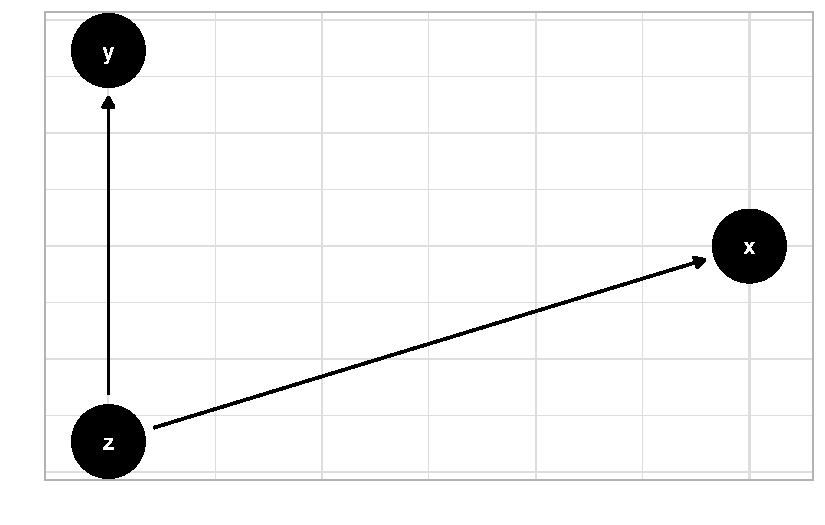
\includegraphics{Papers_beware_collider_files/figure-pdf/fig-basicdag-1.pdf}

}

}

\subcaption{\label{fig-basicdag-1}Fork. Variable z is a common cause of
x and y. You should control for it to avoid ommited variable bias}
\end{minipage}%
%
\begin{minipage}[t]{0.33\linewidth}

{\centering 

\raisebox{-\height}{

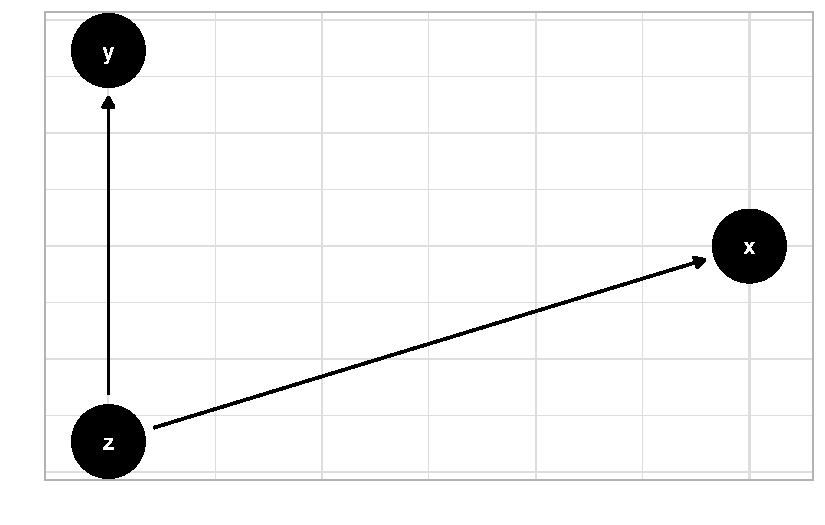
\includegraphics{Papers_beware_collider_files/figure-pdf/fig-basicdag-2.pdf}

}

}

\subcaption{\label{fig-basicdag-2}Chain. Variable x causes z, which
causes y. We say that z is a mediator of thecausal effect of x on y. You
should not control for z.}
\end{minipage}%
%
\begin{minipage}[t]{0.33\linewidth}

{\centering 

\raisebox{-\height}{

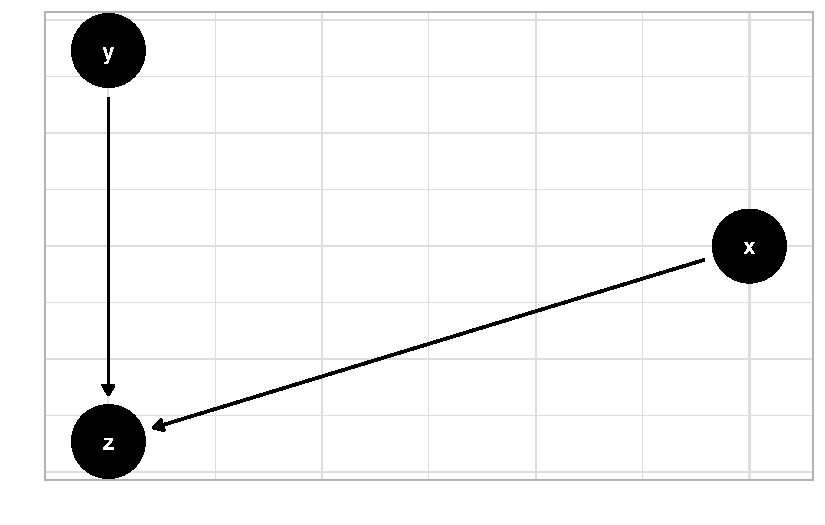
\includegraphics{Papers_beware_collider_files/figure-pdf/fig-basicdag-3.pdf}

}

}

\subcaption{\label{fig-basicdag-3}Invested-fork. Variable z is a common
effect of x and y. Controlling for z opens a backdoor}
\end{minipage}%

\caption{\label{fig-basicdag}Three types of basic DAGs.}

\end{figure*}

All of this means that, if you have a fork, then you should control for
the common variable to avoid omitted variable bias. In that case, we say
that we blocked a backdoor path. If we block all backdoor paths, then
there is no omitted variable bias. Caution is needed when there is a
mediator. If one is interested in the total effect of a variable (say,
\(x\), one the middle chart) on another (\(y\)), then controlling for
the mediator (\(z\)) is wrong, since it will block that specific causal
path. If, on the other hand, one is interested only in the direct
(unmediated) effect, then one should control for the mediator. Last, but
not least, if you are interested in, say, the effect of \(x\) on \(y\)
you should never control for a collider such as \(z\) in the right DAG
above, since it will create a spurious association between variables
(Pearl \& Mackenzie, 2018).

We can then reinterpret the heuristic behind the confound checking
heuristics -- inclusion of controls to deconfound the estimate. It is
trying to block all backdoor paths. However, it says nothing about what
one should do if the control is a mediator or a collider. The focus of
this paper is in the case of inadvertently including a collider.

\hypertarget{a-simple-dag-application-in-the-context-of-tscs}{%
\section{A simple DAG application in the context of
TSCS}\label{a-simple-dag-application-in-the-context-of-tscs}}

To motivate the reader on the usefulness of using a DAG, consider a
common set up in comparative politics in a very simplified setting.
Suppose the researcher is interested in knowing the causal effect of
political regime change on civil war, like in Hegre et. al (2001) that
we quoted when presenting a heuristic for including controls. Suppose,
also, that the only possible (measured) confounder is per capita income
(it can cause civil war and also democratization). Thus, to avoid
omitted variable bias, the researcher decides to control for per capita
income in the regression. Here's the DAG that represents this situation.

\begin{figure}

{\centering 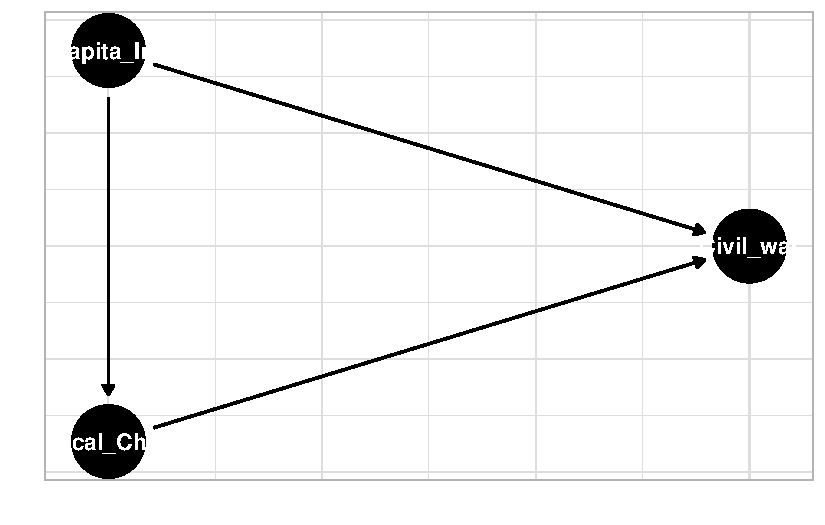
\includegraphics{Papers_beware_collider_files/figure-pdf/fig-dag-model-basic-1.pdf}

}

\caption{\label{fig-dag-model-basic}Simple model of the effect of
poliical change on civil war onset}

\end{figure}

In the context of TSCS data it is standard to index the above variables
by \(t\). For the sake of simplicity, and without loss of generality, we
droped the time tindex by now. Suppose also Suppose that there is
concern about reverse causality, or the fact that it is hard to measure
when a civil war starts. To circumvent such possibilities and make the
results more robust, the researcher decides to lag both per capita
income and political change in the regression.

With such a model in mind and a dataset in the long format, in a
software like R, the researcher would run something like lm(civil\_war
\textasciitilde{} poli\_change\_lag + per\_cap\_income\_lag, data=df)
for a linear probability model and check if the effect is significant.

The software code and the above DAG are deceptively simple. In fact,
they obscure that a dynamic process evolves over time.

Let us unpack what is behind such a dynamic process and how it relates
to a research question by considering a DAG over two periods for the
outcome variable.

\begin{figure}

{\centering 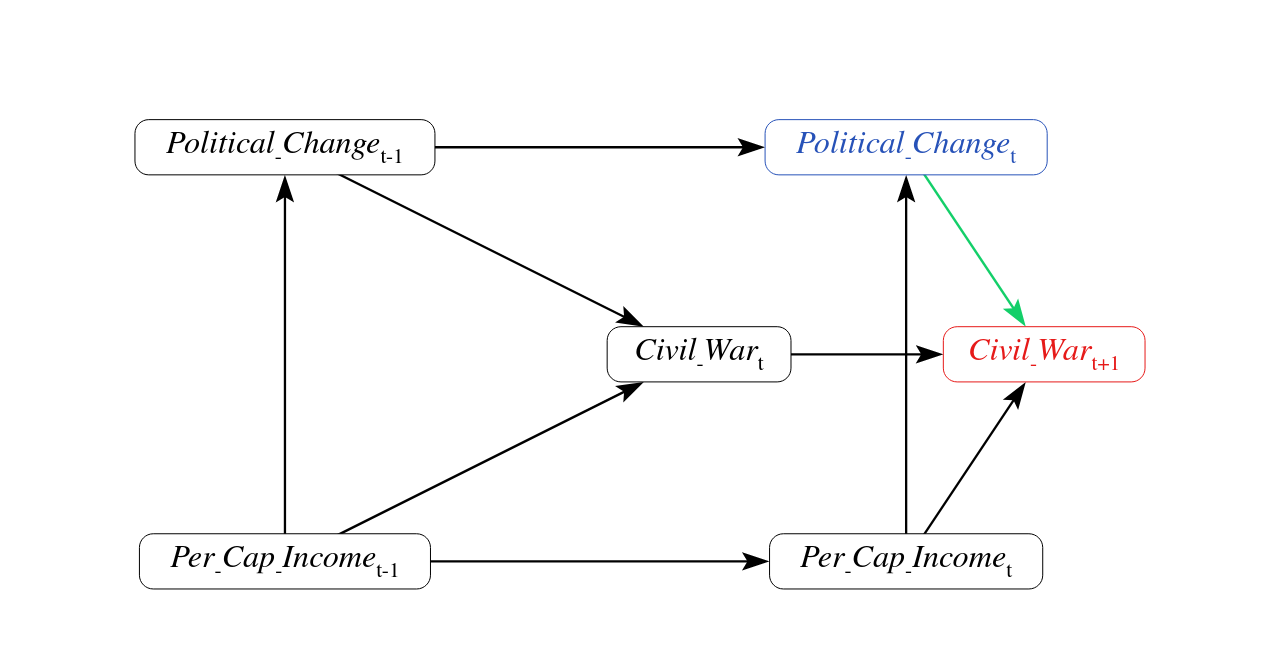
\includegraphics{C:/Users/mczfe/Documents/Papers/Collider TSCS/beware_collider/images/pol change civil war dynamic.png}

}

\caption{DAg civil war dynamic}

\end{figure}

Firstly, in the DAG above, we included arrows from past levels of
variables to current ones. Such a setting is likely in the social
sciences, where persistence and inertia are the norm. In particular, we
know that: per capita income at time t is correlated with its value at
\(t +1\), if there was political change in time \(t\) it will change the
likelihood of another political change in time \(t + 1\). So, a more
believable DAG should include such arrows.

Secondly, it is not easy to say which variable is the treatment or
outcome. In a DAG, both the treatment and the outcome are represented by
a single node. In contrast, we have two nodes that are the treatments:
political change at time \(t -1\) and at time \(t\) and three nodes that
are the outcomes: civil war at \(t -1\), \(t\) and \(t +1\).

To circumvent this in the DAG above, consider only period two. Then, the
causal effect of interest is political change at t on civil war at
\(t +1\). In this case, it is easy to see from the DAG above that there
are two back-doors opened, both going through civil war lagged. Only a
dynamic panel model can recover the actual causal effect.

In this case, whenever there is variation in the treatment effect over
time, the causal effect will be estimated with bias, which will depend
on the distribution of variations of treatment allocation across
countries and time.

We ran a simple simulation based on the above DAG and assumed that civil
war is a normal variable to make things easier to interpret. In every
iteration of the simulation, we kept everything constant but the error
terms and, as a result, who would experience civil war or not in the
end. Other than that, every iteration was the same. There are no
heterogeneous effects over time. The first chart is based on a model in
which only lagged predictors for political change and per capita income
were included. The second chart added a lagged dependent variable to the
model. The true effect of political change on civil war is \(5\).

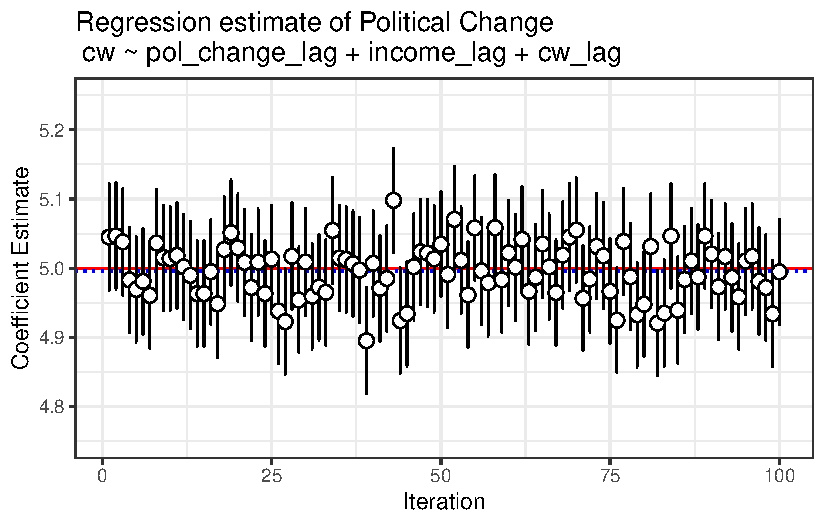
\includegraphics{Papers_beware_collider_files/figure-pdf/simulation 1-1.pdf}

\begin{verbatim}
[1] 10
[1] 20
[1] 30
[1] 40
[1] 50
[1] 60
[1] 70
[1] 80
[1] 90
[1] 100
[1] 110
[1] 120
[1] 130
[1] 140
[1] 150
[1] 160
[1] 170
[1] 180
[1] 190
[1] 200
[1] 210
[1] 220
[1] 230
[1] 240
[1] 250
[1] 260
[1] 270
[1] 280
[1] 290
[1] 300
[1] 310
[1] 320
[1] 330
[1] 340
[1] 350
[1] 360
[1] 370
[1] 380
[1] 390
[1] 400
[1] 410
[1] 420
[1] 430
[1] 440
[1] 450
[1] 460
[1] 470
[1] 480
[1] 490
[1] 500
[1] 510
[1] 520
[1] 530
[1] 540
[1] 550
[1] 560
[1] 570
[1] 580
[1] 590
[1] 600
[1] 610
[1] 620
[1] 630
[1] 640
[1] 650
[1] 660
[1] 670
[1] 680
[1] 690
[1] 700
[1] 710
[1] 720
[1] 730
[1] 740
[1] 750
[1] 760
[1] 770
[1] 780
[1] 790
[1] 800
[1] 810
[1] 820
[1] 830
[1] 840
[1] 850
[1] 860
[1] 870
[1] 880
[1] 890
[1] 900
[1] 910
[1] 920
[1] 930
[1] 940
[1] 950
[1] 960
[1] 970
[1] 980
[1] 990
[1] 1000
\end{verbatim}

\begin{verbatim}
  int_95
1  0.952
\end{verbatim}

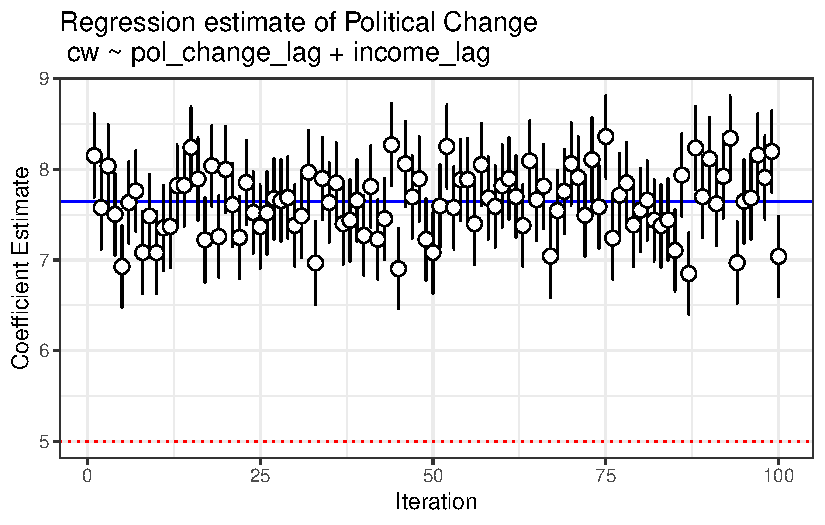
\includegraphics{Papers_beware_collider_files/figure-pdf/simulation 1-2.pdf}

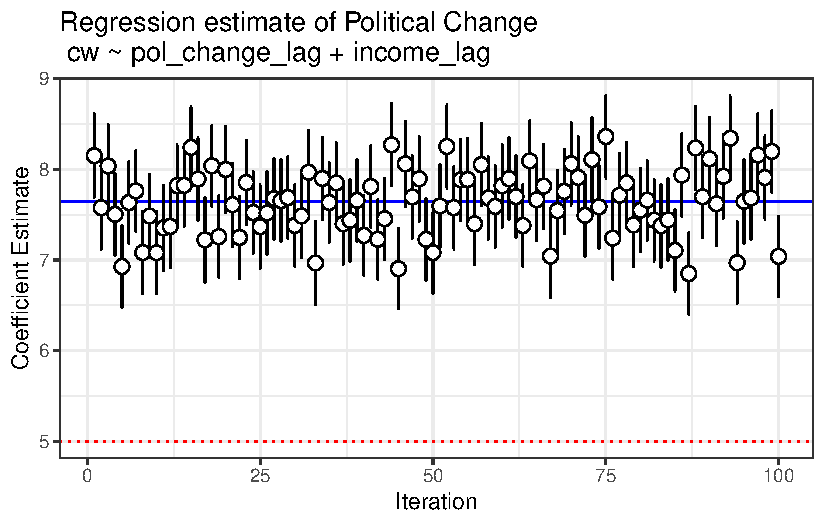
\includegraphics{Papers_beware_collider_files/figure-pdf/simulation 1-3.pdf}

The first model needs to be corrected, but the dynamic panel model is,
on average, correct. Based on the DAG, we already knew that that was the
case. Thus, a DAG can save us much effort and help to specify a model
that can identify a causal effect correctly.

\hypertarget{example-of-back-to-the-futre-collider-bias}{%
\subsection{Example of Back to the futre (collider)
Bias}\label{example-of-back-to-the-futre-collider-bias}}

As mentioned, the problem with including as many controls as possible is
that one may inadvertently include what is called in the Potential
Outcomes framework a ``bad control'' (Angrist \& Pischke, 2009). A bad
control is either a mediator or a collider. The Potential Outcomes
framework provides very generic advice on what is a bad control. When it
is a mediator, the lack of precise advice is not a problem because
knowing that a mediator cannot be a control variable if one is
interested in the total effect is pretty intuitive. However, in the case
of colliders, the intuition should be more straightforward, and we need
a more formal approach, namely, using DAGs.

It is important to note that a collider is only a problem if it is in
the path between the treatment (our x variable) and the outcome (the y
variable). In general, any DAG in a social science context will have
plenty of colliders that create spurious associations between variables.
However, that is not a problem because those associations are not of
interest in a given research. Thus, the DAG is built with a clear goal:
to allow one to check if the causal effect of the treatment on the
outcome is identified. All other causal relations are only important
insofar as they help to identify the causal effect of interest. They are
not of interest per se.

Let us return to our previous example of political change and civil war.
Suppose, like Hegre et al.~(2001), one wants to add other controls to a
regression, such as democracy level. The DAG now is as follows:

\begin{figure}

{\centering 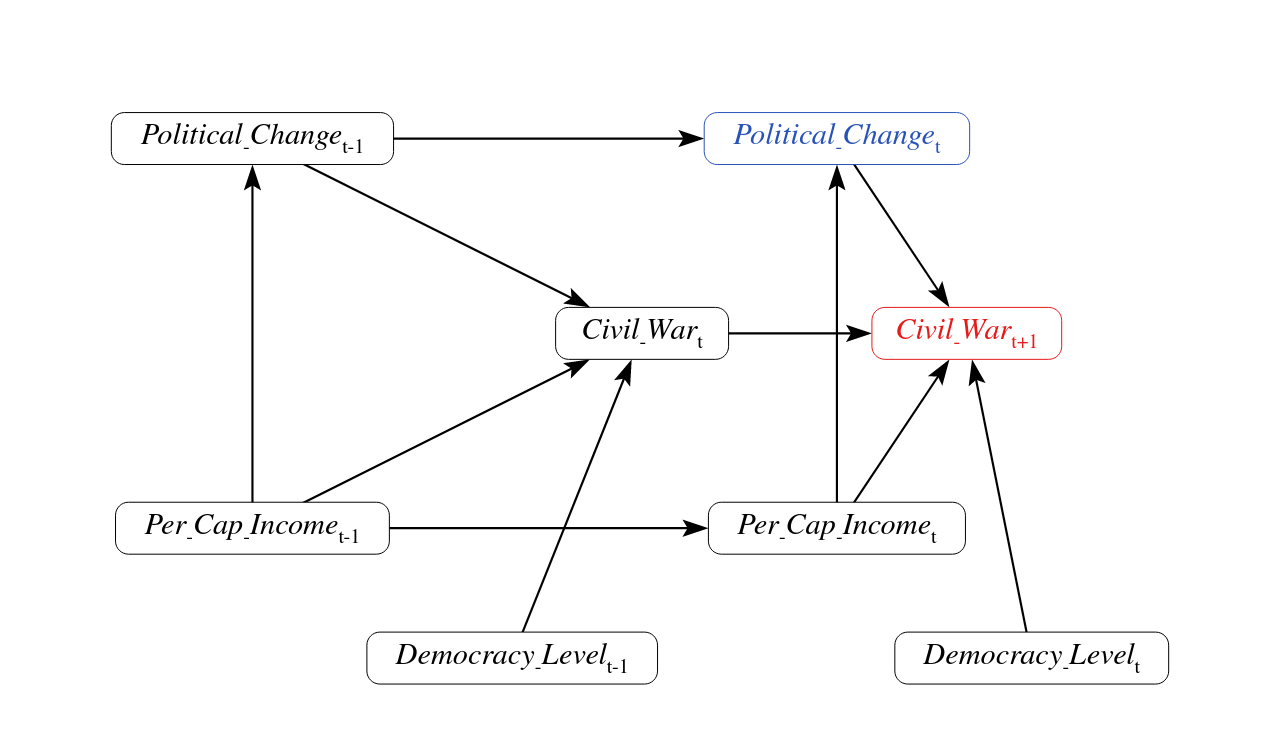
\includegraphics{C:/Users/mczfe/Documents/Papers/Collider TSCS/beware_collider/images/democracy_control.png}

}

\caption{DAg civil war with new control}

\end{figure}

If this is the true DAG, then the model is still identified. We show now
how it is possible to introduce what we call back to the future bias, if
the true DAG (as plausible as the above) is different. We will build it
in steps, to make it clear where the problem resides and how it can
happen.

\hypertarget{step-1-of-back-to-the-future-bias---reverse-causality-of-control-z}{%
\subsection{Step 1 of back to the future bias - reverse causality of
control
z}\label{step-1-of-back-to-the-future-bias---reverse-causality-of-control-z}}

Let's say that after a civil war onset, the democracy level of the
country will likely decrease. In our DAG, this means there is a missing
arrow from current civil war nodes to current democracy levels nodes.
This is know as potential reverse causality, which is dealt with by
lagging the control. Thus. we need to add this arrow and the DAG is now
described by the following graph:

\begin{figure}

{\centering 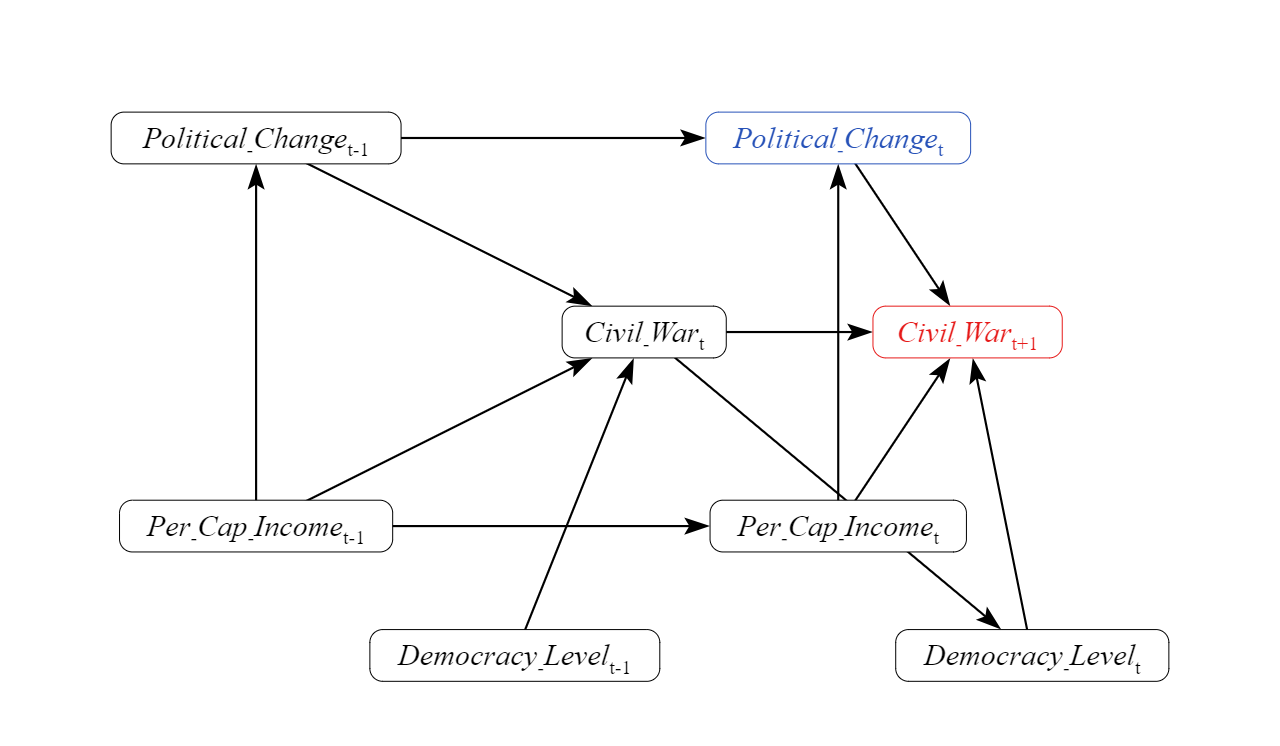
\includegraphics{C:/Users/mczfe/Documents/Papers/Collider TSCS/beware_collider/images/democracy_control_missing_arrow.png}

}

\caption{DAg civil war wit inclusion of missing arrowl}

\end{figure}

\hypertarget{step-2-of-back-to-the-future-bias-treatment-as-cause-of-control-z}{%
\subsection{step 2 of back to the future bias -- treatment as cause of
control
z}\label{step-2-of-back-to-the-future-bias-treatment-as-cause-of-control-z}}

In step 2, the researcher should look at the literature on the causes of
democracy levels. In standard research practice, this never happens,
because according to both control check and confounding checking
heuristics, there is no need to review the literature for potential
causes of the controls included in the regression and include them also
in the regression. We call it foreign literature review, because is a
review of literature not directed related to the research question at
hand, but not another (foreign) research question (that causes a
control?). In any case, let's say she does that and she finds that the
treatment of current research, politcal change, is a cause of democracy
levels, mediated by another variable, not observed in the current study,
\(U\). The new DAG reflecting this potential causal channel is as below:

\begin{figure}

{\centering 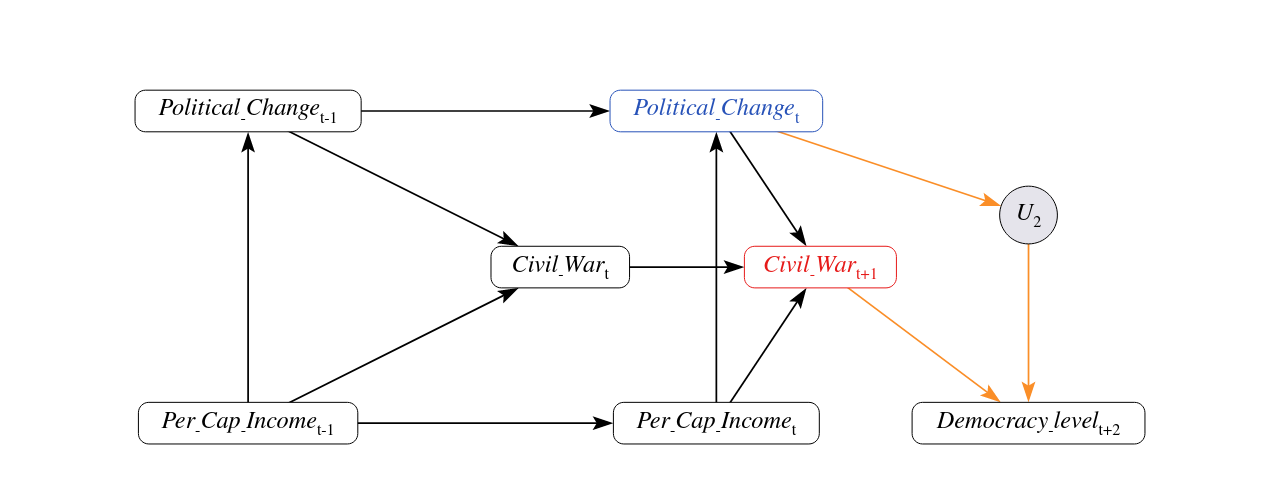
\includegraphics{C:/Users/mczfe/Documents/Papers/Collider TSCS/beware_collider/images/foreign collider bias civil war.png}

}

\caption{back to the future bias - civil war DAG}

\end{figure}

We ommited some arrows from the DAG to make it as simple as possible.
The complete DAG can be found in appendix 1.

The DAG above may be a perfect example of the saying that a picture is
worth a thousand words. In the above DAG, we excluded the past values of
democracy level, causing civil war for simplicity. The variable \(U_2\)
is not included in the regression because no one is concerned about it.
Our standard heuristics suggest including a variable in a regression as
a predictor if it can cause our dependent variable or if it is a
potential source of confounding. On the other hand, the same heuristics
suggest that we should include democracy level because it can cause
civil war (or perhaps is a potential confounding of political change).
However, introducing it as a regressor biases the regression.

To see why it is a collider, notice that democracy level at time \(t+1\)
is a common effect of \(U_2\) and Political Change at time t. By
conditioning on democracy level (including it as a control), we open a
backdoor path connecting \(U_2\) to Civil War.

This problem is specific to TSCS data because of the usage of lagged
variables and the possibility of reverse causality. In the example at
hand, the democracy level variable enters the regression lagged to avoid
reverse causality. However, the reverse causality means there is an
arrow from the dependent variable to current values of democracy level.
If there are any other variables, not observed, caused by police change
that causes current values of democracy level, there is collider bias.

We simulated to show that the previous specification, which did recover
the actual causal effect, fails to do so with the inclusion of a control
variable in the new DAG -- we omitted the arrows from lagged democracy
level to civil war to make things simple.

\begin{verbatim}
[1] 10
[1] 20
[1] 30
[1] 40
[1] 50
[1] 60
[1] 70
[1] 80
[1] 90
[1] 100
[1] 110
[1] 120
[1] 130
[1] 140
[1] 150
[1] 160
[1] 170
[1] 180
[1] 190
[1] 200
[1] 210
[1] 220
[1] 230
[1] 240
[1] 250
[1] 260
[1] 270
[1] 280
[1] 290
[1] 300
[1] 310
[1] 320
[1] 330
[1] 340
[1] 350
[1] 360
[1] 370
[1] 380
[1] 390
[1] 400
[1] 410
[1] 420
[1] 430
[1] 440
[1] 450
[1] 460
[1] 470
[1] 480
[1] 490
[1] 500
[1] 510
[1] 520
[1] 530
[1] 540
[1] 550
[1] 560
[1] 570
[1] 580
[1] 590
[1] 600
[1] 610
[1] 620
[1] 630
[1] 640
[1] 650
[1] 660
[1] 670
[1] 680
[1] 690
[1] 700
[1] 710
[1] 720
[1] 730
[1] 740
[1] 750
[1] 760
[1] 770
[1] 780
[1] 790
[1] 800
[1] 810
[1] 820
[1] 830
[1] 840
[1] 850
[1] 860
[1] 870
[1] 880
[1] 890
[1] 900
[1] 910
[1] 920
[1] 930
[1] 940
[1] 950
[1] 960
[1] 970
[1] 980
[1] 990
[1] 1000
\end{verbatim}

\begin{verbatim}
  int_95
1  0.957
\end{verbatim}

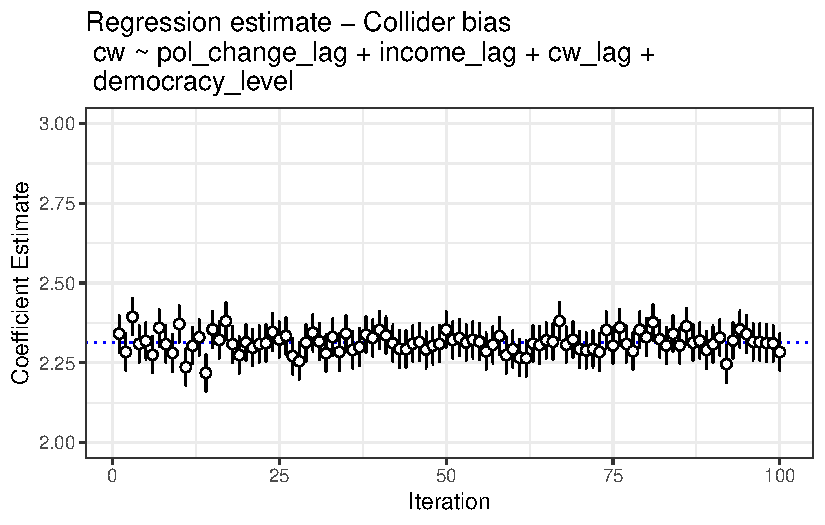
\includegraphics{Papers_beware_collider_files/figure-pdf/simulation 2-1.pdf}

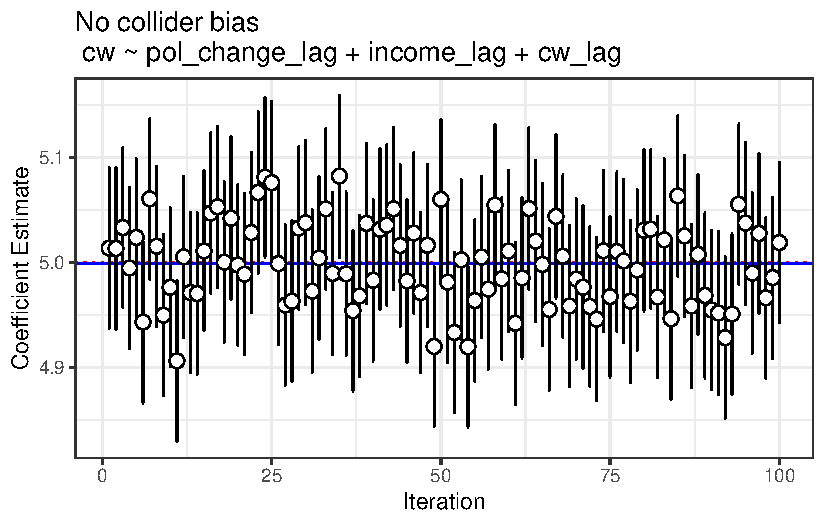
\includegraphics{Papers_beware_collider_files/figure-pdf/simulation 2-2.pdf}

In the chart above, we ran a regression including lagged democracy level
as a control. In the true Data Generating Process (DGP), it did not
cause civil war. However, civil war caused the current values of
democracy level, and an unobserved variable, U, caused democracy level
and was caused by political changThethe DGP was the same in the next
chart. However, we excluded democracy level from the regression. As we
can see, the true causal effect of 5 is recovered on average.

\hypertarget{back-to-the-futue-bias}{%
\section{Back to the futue bias}\label{back-to-the-futue-bias}}

The problem of back to the future bias is not restricted to this
particular case. It is a generic feature os TSCS regression, whenever
some conditions are present, which we provide below:

\hypertarget{the-predictors-are-lagged}{%
\subsection{The predictors are lagged}\label{the-predictors-are-lagged}}

Whenever the predictors as lagged (possibly to avoid reverse causality)
we create the possibility of back to the future collider bias, due to
the fact that we may have a dynamic where
\(x_{t-1} \rightarrow y_t \rightarrow x_t \rightarrow y_{t+1}\). To open
a backdoor previously closed when conditioning on a future collider in
the context of TSCS, it is necessary this dynamic relation Otherwise,
there is no way for a future collider bias the past, so to speaking.

\hypertarget{reverse-causality-from-the-outcome-to-a-control}{%
\subsection{Reverse causality from the outcome to a
control}\label{reverse-causality-from-the-outcome-to-a-control}}

In general we are concerned about reverse causality from the outcome to
the treatment. However, in the case of the back to the future bias, the
problem is reverse causality from the dependent variable on any of the
controls. For each potential reverse causality of this type
(\(y \rightarrow z\), in which \(z\) is a control), together if lagged
predictors we can have back to the future collider bias.

\hypertarget{the-treatment-causes-one-or-more-controls}{%
\subsection{the treatment causes one (or more)
control(s)}\label{the-treatment-causes-one-or-more-controls}}

Lastly, When the main treatment of interest causes one of the controls,
mediated by an unobserved variables or unmeasured variable, in
combination with the two previously condition, necessarily we have back
to the future collider bias. The DAG below (for a one time period
``screen shot'' of a TSCS design) show that this is the case.

\begin{figure}

{\centering 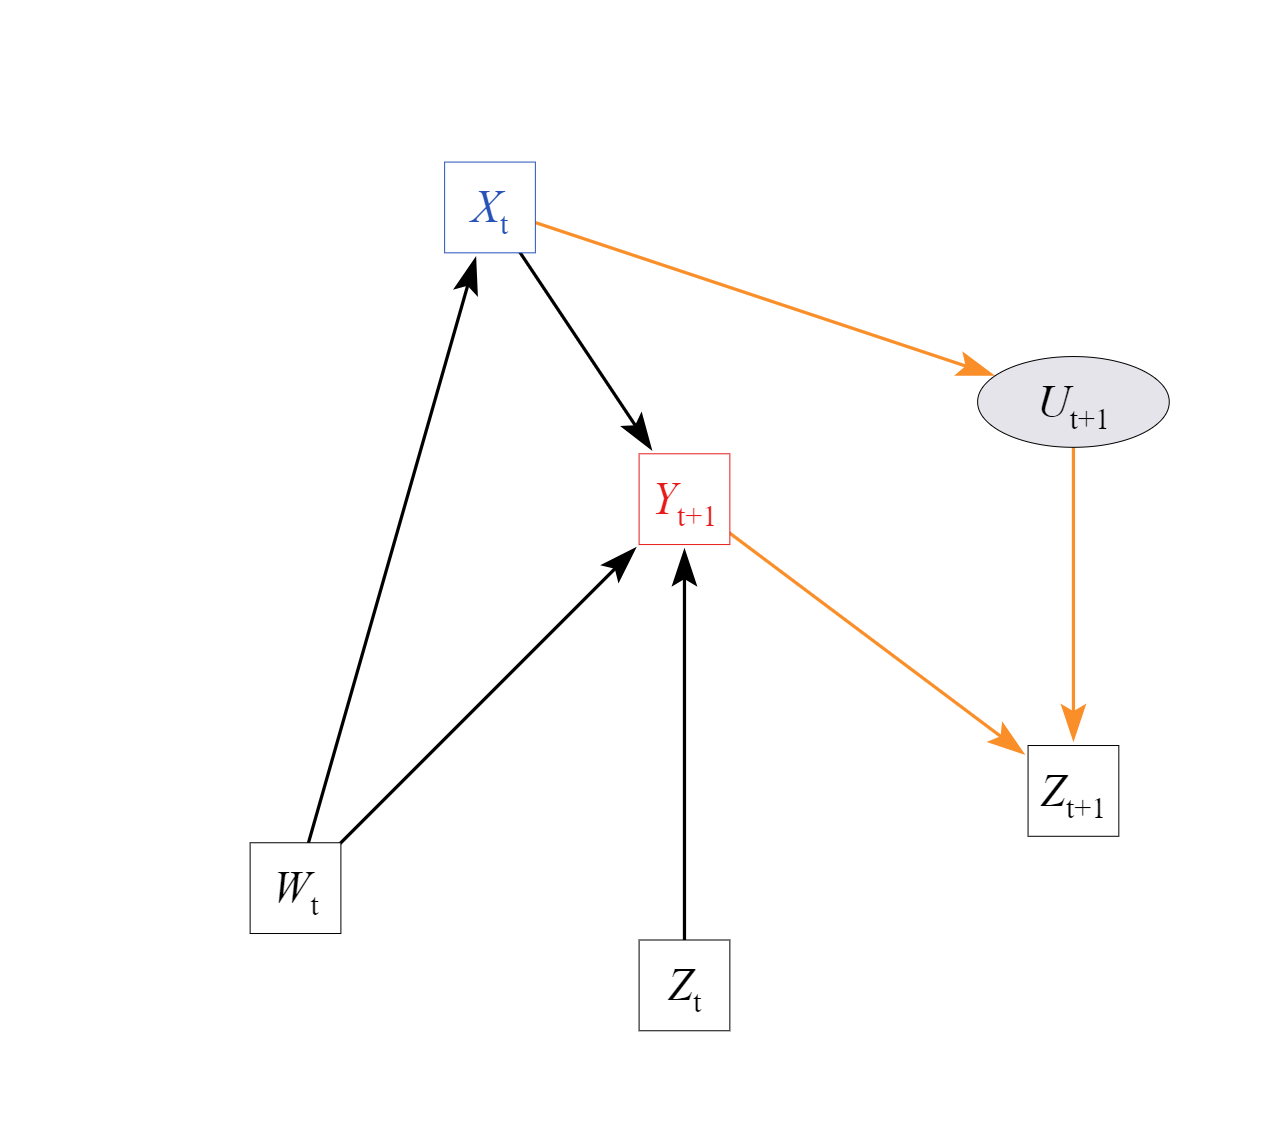
\includegraphics{C:/Users/mczfe/Documents/Papers/Collider TSCS/beware_collider/images/basic_back_future_bias.png}

}

\caption{back to the future bias - one period DAG}

\end{figure}

\hypertarget{tables-coming-from-r}{%
\section{Tables coming from R}\label{tables-coming-from-r}}

Tables can also be generated using R chunks, as shown in
Table~\ref{tbl-simple} example.

\begin{Shaded}
\begin{Highlighting}[]
\NormalTok{knitr}\SpecialCharTok{::}\FunctionTok{kable}\NormalTok{(}\FunctionTok{head}\NormalTok{(mtcars)[,}\DecValTok{1}\SpecialCharTok{:}\DecValTok{4}\NormalTok{])}
\end{Highlighting}
\end{Shaded}

\hypertarget{tbl-simple}{}
\begin{longtable}[]{@{}lrrrr@{}}
\caption{\label{tbl-simple}Caption centered above table}\tabularnewline
\toprule\noalign{}
& mpg & cyl & disp & hp \\
\midrule\noalign{}
\endfirsthead
\toprule\noalign{}
& mpg & cyl & disp & hp \\
\midrule\noalign{}
\endhead
\bottomrule\noalign{}
\endlastfoot
Mazda RX4 & 21.0 & 6 & 160 & 110 \\
Mazda RX4 Wag & 21.0 & 6 & 160 & 110 \\
Datsun 710 & 22.8 & 4 & 108 & 93 \\
Hornet 4 Drive & 21.4 & 6 & 258 & 110 \\
Hornet Sportabout & 18.7 & 8 & 360 & 175 \\
Valiant & 18.1 & 6 & 225 & 105 \\
\end{longtable}

\hypertarget{equations}{%
\section{Equations}\label{equations}}

Here is an equation: \[ 
  f_{X}(x) = \left(\frac{\alpha}{\beta}\right)
  \left(\frac{x}{\beta}\right)^{\alpha-1}
  e^{-\left(\frac{x}{\beta}\right)^{\alpha}}; 
  \alpha,\beta,x > 0 .
\]

Inline equations work as well: \(\sum_{i = 2}^\infty\{\alpha_i^\beta\}\)

Please make sure that your manuscript follows the guidelines in the
Guide for Authors of the relevant journal. It is not necessary to
typeset your manuscript in exactly the same way as an article, unless
you are submitting to a camera-ready copy (CRC) journal.

For detailed instructions regarding the elsevier article class, see
\url{https://www.elsevier.com/authors/policies-and-guidelines/latex-instructions}

\hypertarget{bibliography-styles}{%
\section{Bibliography styles}\label{bibliography-styles}}

Here are two sample references: \citet{Feynman1963118}
\citet{Dirac1953888}.

By default, natbib will be used with the \texttt{authoryear} style, set
in \texttt{classoption} variable in YAML. You can sets extra options
with \texttt{natbiboptions} variable in YAML header. Example

\begin{verbatim}
natbiboptions: longnamesfirst,angle,semicolon
\end{verbatim}

There are various more specific bibliography styles available at
\url{https://support.stmdocs.in/wiki/index.php?title=Model-wise_bibliographic_style_files}.
To use one of these, add it in the header using, for example,
\texttt{biblio-style:\ model1-num-names}.

\hypertarget{using-csl}{%
\subsection{Using CSL}\label{using-csl}}

If \texttt{cite-method} is set to \texttt{citeproc} in
\texttt{elsevier\_article()}, then pandoc is used for citations instead
of \texttt{natbib}. In this case, the \texttt{csl} option is used to
format the references. By default, this template will provide an
appropriate style, but alternative \texttt{csl} files are available from
\url{https://www.zotero.org/styles?q=elsevier}. These can be downloaded
and stored locally, or the url can be used as in the example header.


\renewcommand\refname{References}
  \bibliography{bibliography.bib}


\end{document}
